% Chapter 1
\stepcounter{cap}
%\chapter{cap1}
\label{cap3}

\mychapter{3}{Capitolul \arabic{cap} \\ ARHITECTURA SOFTWARE}
%\chapter{\arabic{cap}.Introducere} % Main chapter title

\label{Chapter3} % For referencing the chapter elsewhere, use \ref{Chapter1} 

\thispagestyle{fancy}

%-----------------------------------------------------------------
În acest capitol este prezentată partea structurală a modulului cât şi unităţile software din care acesta este format.

\section{Limbajul C++}
Limbajul de programare C++ reprezintă de fapt o vastă colecție de comenzi folosite pentru controlul computerelor, numite și cod.
\vspace{6pt}
\\C++ este un limbaj de programare orientat pe obiecte ce a fost dezvoltat ca o extensie a originalului limbaj C în anul 1980. Este considerat a avea un nivel de dificultate intermediar, deoarece acoperă atât funcții de nivel înalt cât și de nivel scăzut.
\vspace{6pt}
\\Potrivit Fundației C++ Standard, limbajul oferă un sitem de memorie sistemică și un calcul structural ce seamănă foarte mult cu programarea celor mai multe computere. Acesta este folosit la o multitudine de sarcini, de la extragerea datelor din bazele de date la afișarea graficii jocurilor video sau chiar la controlarea dispozitivelor electronice atașate computerului.
\vspace{6pt}
\\Deoarece poate fi folosit pe orice sistem de operare, C++ este un limbaj de programare universal ce este găsit pe majoritatea computerelor.

\subsection{Obiectivele de proiectare}
C++ a fost inițial creat de Bjarne Stroustrup în cadrul Laboratoarelor AT\&T Bell, ca o cale de a depasi limitările limbajelor de programare deja existente, precum C și Simula.
\vspace{6pt}
\\C++ a fost creat cu scopul de a oferi flexibilitate, eficiență și o organizare structurală. În mod specific, mecanismele de încorporare abstractă au fost proiectate pentru a face față celor mai dificile și solicitante sarcini de programare.
\vspace{6pt}
\\C++ suportă abstractizarea datelor, programarea generică dar și programarea orientată pe obiecte. Deoarece c++ a fost gândit pentru a fi un limbaj de programare cu scop general, este foarte ușor de folosit și de utilizat.

\subsection{Funcționalitate multiplă}
C++ este foarte popular deoarece este extrem de funcțional. Este folosit pentru a crea sisteme de operare, drivere de dispozitiv și protocoale de rețea.
\vspace{6pt}
\\Este de asemenea utilizat pentru a dezvolta aplicații pentru baze de date, foi de calcul și procesare de text. Deoarece este un limbaj cu scop general, este potrivit pentru dezvoltarea oricărui tip de software. Acest lucru este posibil prin intermediul a peste 10 sisteme unice de implementare și sute de biblioteci, manuale și jurnale tehnice.
\vspace{6pt}
\\Deoarece C ++ permite programatorilor să creeze rapid programe în limite urgente de timp și spațiu, C ++ este ideal pentru manipulări hardware directe în constrângeri în timp real. Într-un astfel de cod, previzibilitatea performanței este cel puțin la fel de importantă ca și viteza brută.
\vspace{6pt}
\\Fiabilitatea C ++ a dus la favorizarea organizațiilor de tranzacționare, bancare, de asigurări, militare și de telecomunicații. 

\subsection{Avantaje}
C ++ este un limbaj foarte portabil, ceea ce înseamnă că programatorii pot scrie programe indiferent de limitele hardware și de sistemul de operare. Ca rezultat, programatorii pot dezvolta un program inițial care este tradus sistematic pe diferite platforme.
\vspace{6pt}
\\Orice program care a fost dezvoltat în limbajul original C poate fi ușor mutat în C ++ fără modificări majore. Deoarece C ++ oferă flexibilitate, programatorii sunt capabili să creeze construcții puternice și să introducă noi obiecte conceptuale și aplicații abstracte.
\vspace{6pt}
\\Ca rezultat, C ++ permite programatorilor să controleze și să manipuleze resursele hardware pentru a produce programe de funcționare înalte. C ++ vine cu câteva dezavantaje, cum ar fi numeroase erori de securitate și funcționalitate slabă a dezvoltării web.
\vspace{6pt}
\\Limbajul de programare C ++ este astfel unul din limbajele cele mai utilizate și versatile pe care toți începătorii ar trebui să-l învețe.

\section{Enterprise Architect} 
Sparx Systems Enterprise Architect este un instrument de modelare vizuală și de proiectare bazat pe OMG UML.
\vspace{6pt}
\\Platforma suportă: proiectarea și construirea de sisteme software, modelarea proceselor de afaceri, și modelarea domeniilor bazate pe industrie.
\vspace{6pt}
\\Este folosită de întreprinderi și de organizații nu numai pentru să modelarea arhitecturii sistemelor lor, ci și pentru a procesa implementarea acestor modele în întregul ciclu de viață al dezvoltării aplicațiilor.
\vspace{6pt}
\\Enterprise Architect este construit pe baza specificațiilor UML 2.
\vspace{6pt}
\\Utilizarea profilelor UML extinde capabilitățile de modelare iar validarea modelelor garantează integritatea.
\begin{figure}[h!]
  \centering
   \centering{%
   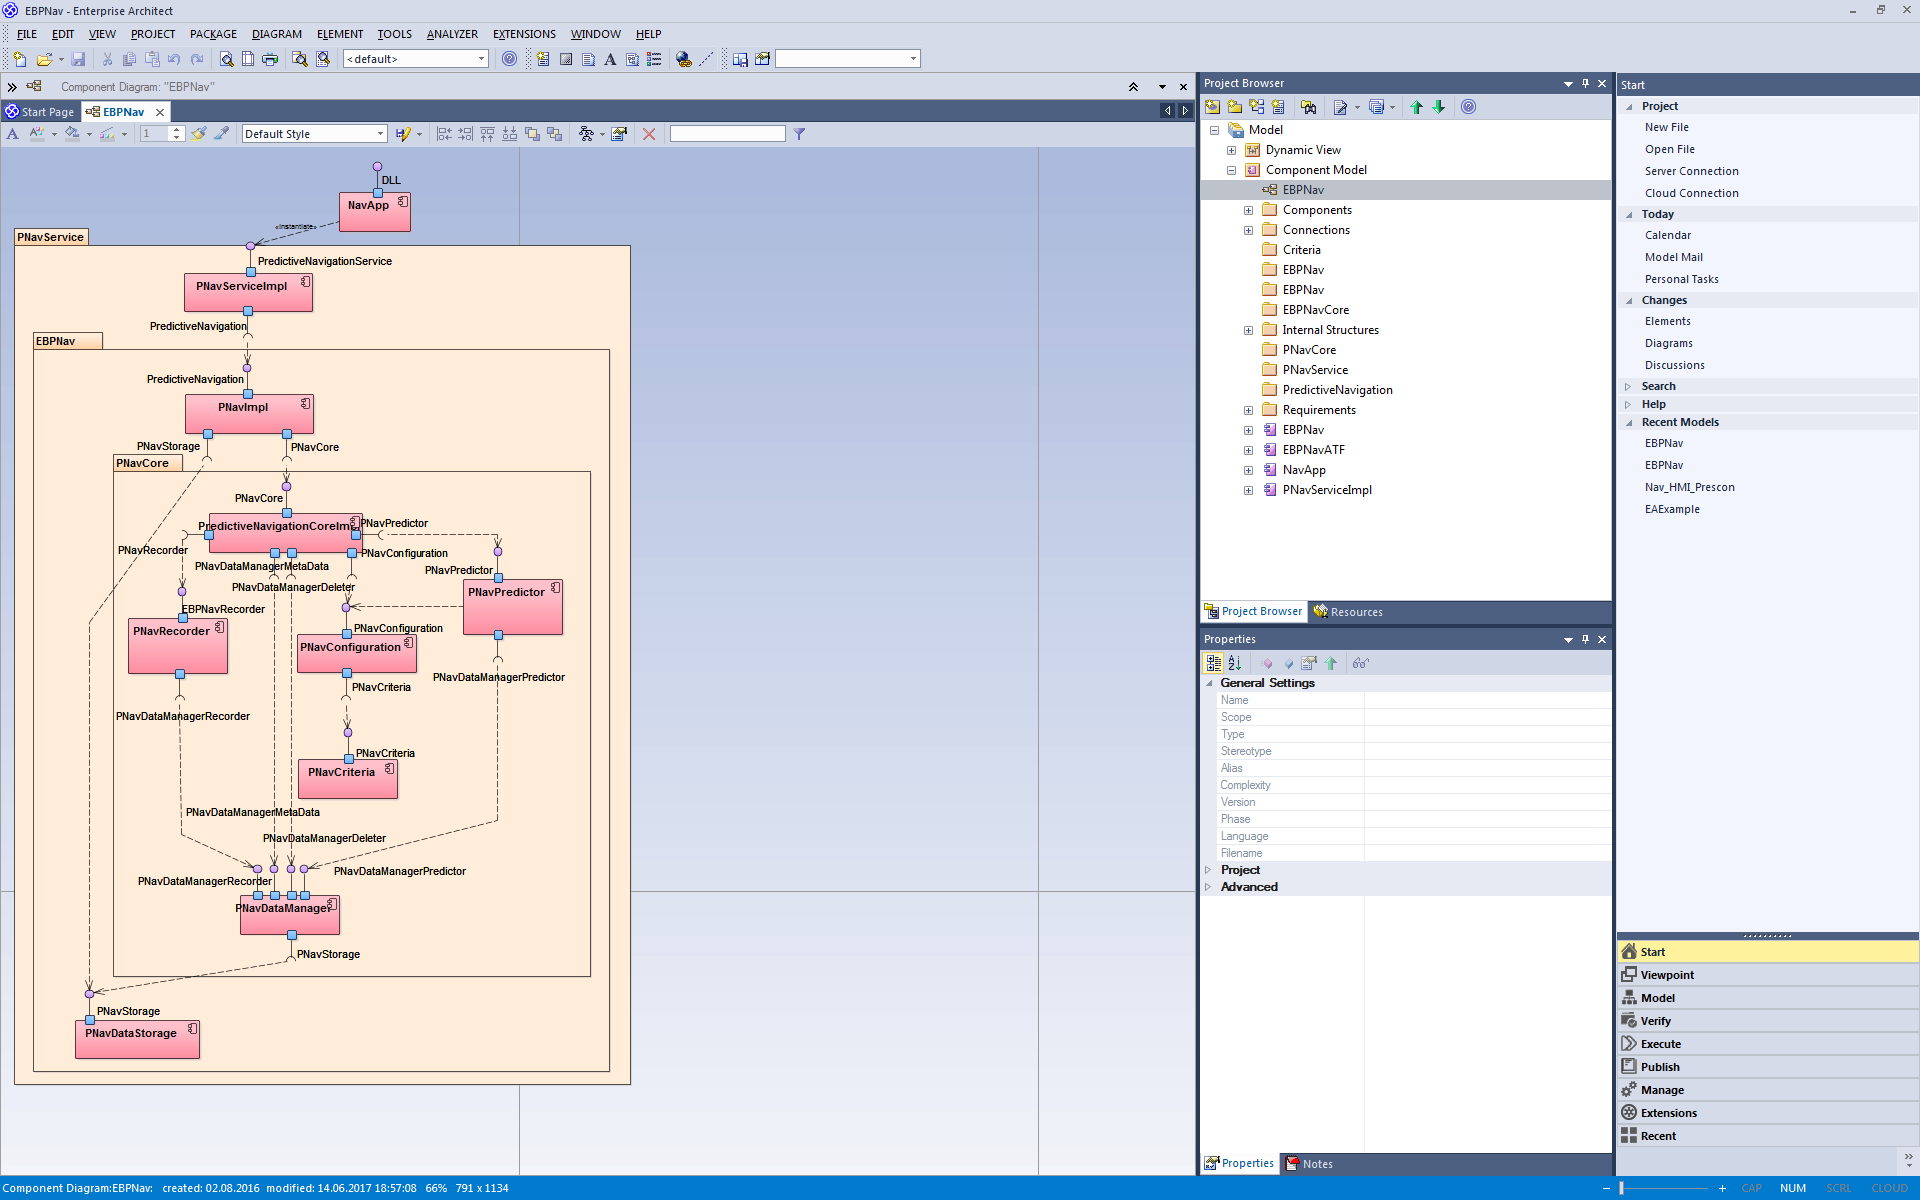
\includegraphics[width=0.9\textwidth]{Figures/ea.png}}
  \caption{Captură de ecran din Enterprise Architect}
  \end{figure}	

\subsection{Diagramele UML}
UML este o modalitate de vizualizare a unui program software folosind o colecție de diagrame.
\vspace{6pt}
\\Notația a evoluat de la munca lui Grady Booch, James Rumbaugh, Ivar Jacobson și Rational Software Corporation pentru a fi folosită pentru design orientat pe obiecte, dar de atunci a fost extinsă pentru a acoperi o varietate mai largă de proiecte de inginerie software. Astăzi, UML este acceptat de către Grupul de Management al Obiectului(OMG) ca standard pentru modelarea dezvoltării de software.
\vspace{6pt}
\\Termenul de UML vine de la Unified Modeling Language (limbaj unificat de modelare). UML 2.0 a ajutat la extinderea specificației UML originale pentru a acoperi o parte mai mare a eforturilor de dezvoltare software, inclusiv practicile Agile.
\vspace{6pt}
\\Deși este folosit în mod obișnuit în ingineria software, este un limbaj bogat care poate fi folosit pentru a modela structurile de aplicații, comportamentul și chiar procesele de afaceri. Există 14 tipuri de diagrame UML care vă ajută să modelați aceste comportamente, ele putând fi împărțite în două categorii principale; Diagrame structurale și diagrame comportamentale. 

	\begin{itemize}
	 \setlength\itemsep{0em}
		\item Diagramă tip clasă
		\item Diagramă tip componentă
		\item Diagramă de implementare
		\item Diagramă tip obiect	
		\item Diagramă tip pachet 
		\item Diagramă tip profil
		\item Diagramă tip structură compozită
		\item Diagramă tip scenariu
		\item Diagramă de activitate
		\item Diagramă tip stare mașină
		\item Diagramă de secvență
		\item Diagramă de comunicare
		\item Diagramă de interacțiune generală
		\item Diagramă de timp
	\end{itemize}


\begin{figure}[h!]
  \centering
   \centering{%
   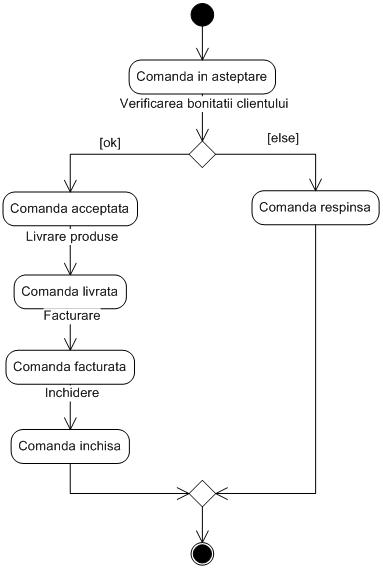
\includegraphics[width=0.5\textwidth]{Figures/diagrama_uml.jpg}}
  \caption{Diagramă de tip statechart pentru cazul realizării unei comenzi}
  \end{figure}	

\section{Deciderea asupra comportamentului sincron și asincron} 
	Fiecare mod de executare a operațiilor are propriile sale avantaje și dezavantaje.
	Există operaţii care ar putea necesita mai mult timp pentru a se termina de executat (>100ms) şi nu este direct vizibil faptul dacă acestea au fost declanşate de către o cerere (e.g. o  nouă poziţie este trimisă).
	\vspace{6pt}
    \\O cerere poate declanşată din fire de execuţie diferite.
	Există posibilitatea ca acest lucru sa fie realizat sincron, în afara modului, între cereri şi răspunsuri, fapt ce poate duce la deadlock.

	\subsection{Factori de decizie} 
	\begin{itemize}
	 \setlength\itemsep{0em}
		\item Timpul în care firul de execuţie este blocat de cerere
		\item Sincronizarea între operaţii
	\end{itemize}

	\subsection{Soluţii propuse}
	\begin{itemize}
	 \setlength\itemsep{0em}
		\item Procesul se va executa asincron folosind un fir de execuţie de lucru
		\item Procesul se va executa sincron, în interiorul cererilor
	\end{itemize}


	\subsection{Decizia}
	Se vor furniza două interfeţe diferite. Funcţionalitatea va fi oferită printr-o interfaţă sincronă, ce va fi utilizată în cadrul operaţiilor ce au loc pe un singur fir de execuţie. O altă interfaţă va decupla firele de execuţie şi procesele din bucla de lucru.
	Acest fapt ne oferă libertatea utilizării principiului de multithread-ing (execuţia mai multor thread-uri în acelaşi pipeline, fiecare având propria secţiune de timp în care este menit să lucreze).
\clearpage 

\section{Structura modulului din punctul de vedere al unităților software}
\begin{figure}[h!]
  \centering
   \centering{%
   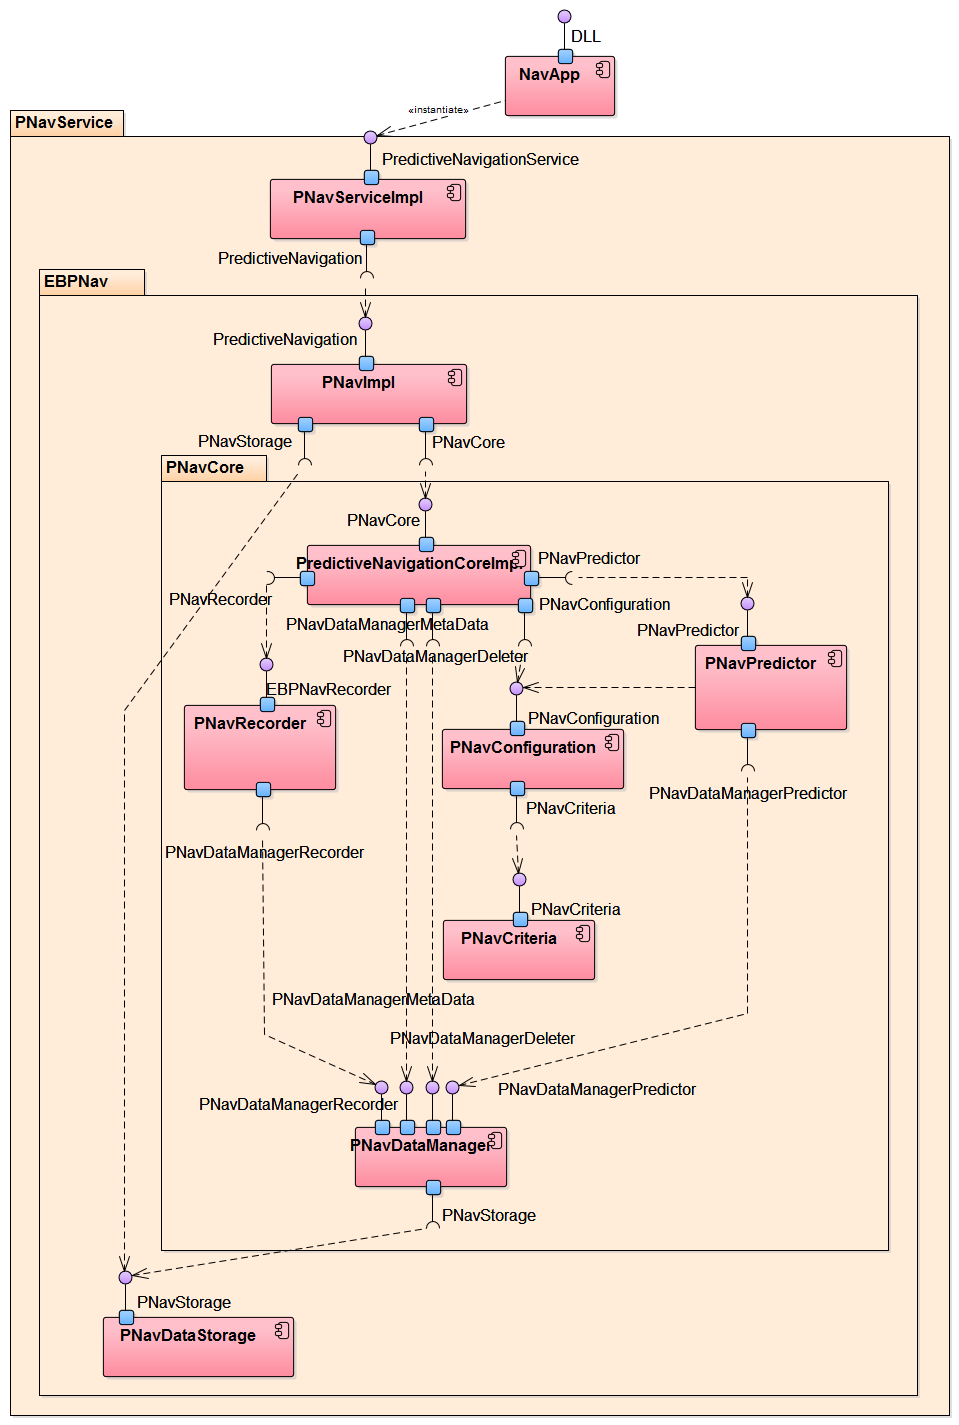
\includegraphics[width=0.8\textwidth]{Figures/pnav.png}}
  \caption{Diagrama componentelor}
  \end{figure}	
  
\subsection{Unitatea software PNavDLL} 
Această unitate realizează "ambalarea" întregului modul sub forma unei biblioteci cu legare dinamică (\acrfull{dll}).

\subsection{Unitatea software PNavCoreImpl} 
Unitatea PNavCoreImpl are rol de dispecer, utilizând restul unităților pentru realizarea funcționalităților de bază. 

\subsection{Unitatea software PNavServiceImpl} 
Unitatea PNavServiceImpl implementează interfaţa sincronă şi asincronă, şi îi oferă totodată dezvoltatorului posibilitatea de a alege ce interfaţă doreşte să folosească.
\vspace{6pt}
\\Cea asincronă are avantajul de a decupla firele de execuţie şi de a permite rularea activităţilor în paralel, însă are şi dezavantajul necesităţii de implementare unui mecanism de sincronizare în codul aplicaţiei în care va fi folosit modulul.


\subsection{Unitatea software PNavImpl} 
Deşi funcţionalităţile de bază precum precum învăţarea şi predicţia sunt realizare de către unitatea PNavRecorder respectiv PNavPredictor, unitatea PNavImpl realizează funcţionalităţi suplimentare cum ar fi multiple profile de utilizatori, ştergerea bazelor de date.
\vspace{6pt}
\\Funcţionalitatea multiplelor profile de utilizatori permite gestionarea mai multor baze de date, ce pot fi selectate pe baza unui ID de profil.
Acest ID poate cuprinde valori în intervalul 0-255. Pentru fiecare profil este creat un nou fişier în care vor fi stocate datele de utilizator. Unitatea PNavImpl implementează de asemenea şi funcţionalităţi de întreţinere a profilelor de utilizator precum ştergerea individuală, ştergerea totală, copierea, schimbarea între profile.

\subsection{Unitatea software PNavRecorder} 
NavRecorder-ul este unitate în care întreg procesul de învăţare are loc. 
\vspace{6pt}
\\Unitatea primeşte datele de geolocație şi de timp (oră - zi/lună/an) şi învaţă rutele parcurse de către dezvoltator într-un mod inteligent.
Acest lucru înseamnă că waypoint-urile (punctele prin care a trecut utilizatorul în timpul rutei sale) sunt stocate numai când autovehiculul şi-a schimbat 
orientarea semnificativ (valoare standard: > 15$^{\circ}$) sau distanţa dintre waypoint-uri nu este prea scurtă (valoare standard: > 200m). Valori pot fi configurate înaintea procesului de compilare.
\vspace{6pt}
\\Când sesiunea de înregistrare este finalizată, waypoint-urile sunt trimise către unitatea software PNavDataManager pentru a fi scrise în baza de date.
Totodată, unitatea are implementate funcţionalităţi de oprire-pornire, lucru ce-i acordă dezvoltatorului dreptul de opri şi porni oricând sesiunea de înregistrare.


\subsection{Unitatea software PNavPredictor} 
Rolul unităţii PNavPredictor este acela de a calcula predicţiile. 
\vspace{6pt}
\\Primul pas constă în încărcarea datelor prin unitatea PNavDataManager, care sunt mai departe prioritizate în funcţie de criterii specifice (descrise în tabela ~\ref{table:tabel_predictii}, ``Criterii de prioritizare pentru predicţia bazată pe rute''). Datele pot fi de asemenea filtrate pe baza aceloraşi criterii, rezultând astfel o cantitate mai mică de date şi un timp mai scurt de încărcare a acestora. 
\vspace{6pt}
\\Prioritizarea datelor este bazată atât pe datele de geolocație cât şi cele de timp, astfel încât o rută va avea o probabilitate mult mai mare de utilizare într-o anumită zi din săptămână sau la o anumită oră din zi.
\vspace{6pt}
\\Ca şi unitatea PNavRecorder, unitatea PNavPredictor are implementate funcţionalităţi de oprire-pornire.


\subsection{Unitatea software PNavConfiguration} 
Unitatea PNavConfiguration configurează unitatea NavPredictor, prin intermediul unor funcţii ce folosesc criteriile definite în unitatea PNavCriteria.


\subsection{Unitatea software PNavCriteria} 
Unitatea PNavCriteria conţine toate tipurile de criterii ce pot fi folosite la filtrarea sau prioritizarea datelor.
\vspace{6pt}
\\Fiecare criteriu în parte este folosit la procesarea datelor de către unitatea PNavPredictor.
După procesarea tuturor criteriilor cea mai probabilă rută este creată.


\subsection{Unitatea software PNavDataManager} 
Unitatea PNavDataManager implementează logica necesară pentru a realiza comunicarea între unitatea PNavDataStorage şi restul unităţilor.
\vspace{6pt}
\\În general, obiectele sunt stocate separat (e.g. rutele sunt stocate separat faţă de destinaţiilor lor). Cum însă pentru predicţia unei rute este nevoie de toate informaţiile, unitatea PNavDataManager le comasează. Aceasta oferă de asemenea şi alte funcţionalităţi precum adăugarea, gruparea, căutarea sau ştergerea de obiecte.


\subsection{Unitatea software PNavDataStorage} 
Unitatea PNavDataStorage este dezvoltată pe baza structurii bazei de date.
\vspace{6pt}
\\În afară de funcţionalitatea principală de a stoca sau încărca date, aceasta asigură şi accesarea selectivă a obiectelor. Pentru realizarea acestor funcţionalităţi se execută interogări prin intermediul SQLite.
